\chapter{System Design}

ProblySUS employs a modular client-server architecture designed for scalability, maintainability, and efficient data exchange. The client layer accepts a URL as input either typed into the web application or automatically read from the active browser tab via the Chrome extension and submits it to the backend analysis pipeline, ensuring a fast and accessible experience across devices.

\textbf{Main Components}

The system consists of three primary layers: Input, Processing, and Output.

The \textbf{Input Layer} includes the web frontend URL input bar and the browser extension popup, both capable of accepting any syntactically valid URL.

The \textbf{Processing Layer} consists of the Flask backend orchestrating ten analysis modules covering domain intelligence, DNS checks, URL pattern analysis, content inspection, blacklist lookup, headless browser simulation, network classification, privacy auditing, and tracker identification. All module outputs are aggregated by a central scoring engine.

The \textbf{Output Layer} delivers a structured JSON risk report rendered as an interactive results dashboard containing a score gauge, risk label, reasons list, and detailed analysis panels.

On the server side, the system manages URL validation, parallel execution of analysis modules, threat intelligence lookups, result caching, and auto-updating of the local blacklist feed. All outputs are returned to the client as a single structured JSON response consumed by both the web frontend and the browser extension. The architecture requires no user authentication since no personal data is stored. Only URL scan results are temporarily cached in memory for 30 minutes.

\section{Overall System Architecture Flowchart}

Figure~\ref{fig:overall_architecture_flow} provides a high-level flowchart of the complete ProblySUS workflow from URL submission to final risk presentation. It shows how user input is validated, distributed to parallel analysis modules, merged by the scoring engine, and then returned to both client interfaces.

\begin{figure}[!htbp]
\centering
\fbox{%
\begin{minipage}{0.95\textwidth}
\centering
\textbf{User Sources}\\[3pt]
Web App URL Input \quad + \quad Chrome Extension Active Tab\\[8pt]
$\downarrow$\\[8pt]
\textbf{Input Validation Layer}\\[3pt]
URL normalization, syntax checks, HTTPS/TLS verification\\[8pt]
$\downarrow$\\[8pt]
\textbf{Parallel Analysis Pipeline}\\[3pt]
WHOIS \;|\; DNS \;|\; URL Pattern \;|\; Content \;|\; Blacklist\\
Behavior \;|\; Network \;|\; Privacy \;|\; Tracker Detection\\[8pt]
$\downarrow$\\[8pt]
\textbf{Aggregation and Scoring Engine}\\[3pt]
Weighted penalties, compound signals, risk label generation\\[8pt]
$\downarrow$\\[8pt]
\textbf{Response and Presentation Layer}\\[3pt]
Structured JSON report $\rightarrow$ Dashboard + Extension Tabs\\
\end{minipage}%
}
\caption{Overall System Architecture Flowchart of ProblySUS}
\label{fig:overall_architecture_flow}
\end{figure}

This flowchart clarifies the control flow and data flow across all major components. It highlights that ProblySUS does not rely on a monolithic scan step; instead, it runs specialized modules in parallel and fuses their outputs into one explainable and user-friendly result.

\section{Data Flow Diagram (DFD)}

The Data Flow Diagram illustrates how data moves from the user to the analysis modules and finally to the generated risk report. When a user submits a URL through the web application or browser extension, the system validates the URL and distributes it across multiple analysis modules operating in parallel.

Each module independently analyzes a particular signal domain and returns structured results. These results are then aggregated by the scoring engine to compute the final composite risk score and generate a labeled report returned to the client interface.

The following figure illustrates the operational data path of a scan request in detail. It emphasizes how the same input URL is propagated to multiple analysis modules, then consolidated into a single report, ensuring both analytical depth and consistent output formatting.

\begin{figure}[!htbp]
\centering
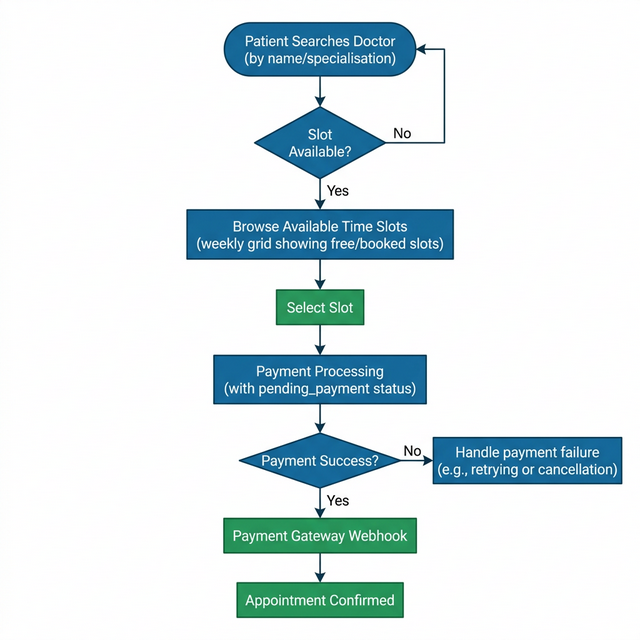
\includegraphics[width=0.85\textwidth]{images/chapter4/dfd_problysus.png}
\caption{Data Flow Diagram of ProblySUS}
\label{fig:dfd_problysus}
\end{figure}

\section{Use Case Diagram}

The Use Case Diagram defines interactions between users and the system.

ProblySUS has a single primary user role called the \textbf{End User}. The end user can perform the following actions:

\begin{itemize}
\item Submit a URL for analysis
\item View the risk report including score, label, and explanation
\item Inspect behavior, network, privacy, and tracker panels
\item Trigger manual blacklist update
\item Open the full web report from the browser extension
\end{itemize}

Additionally, the system includes a background component known as the \textbf{System Daemon}. This component automatically refreshes the blacklist feed every 24 hours without requiring user interaction.

\begin{figure}[!htbp]
\centering
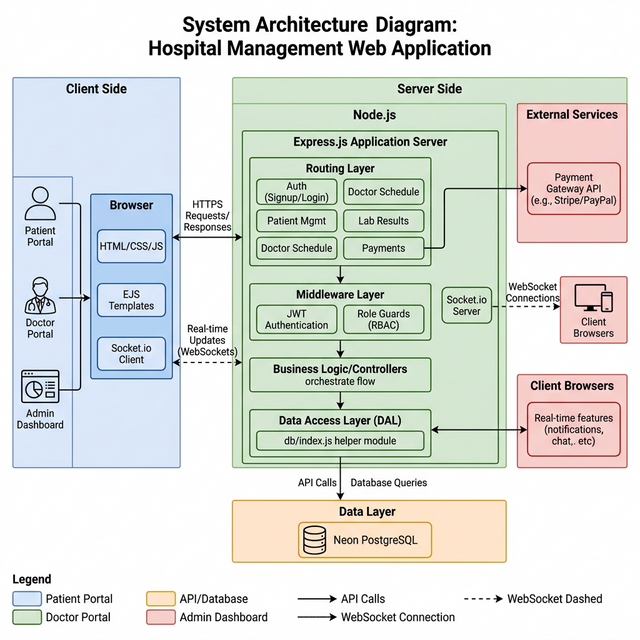
\includegraphics[width=0.75\textwidth]{images/chapter4/usecase_problysus.png}
\caption{Use Case Diagram of ProblySUS}
\label{fig:usecase_problysus}
\end{figure}

This use case view clarifies user-facing functionality and background automation responsibilities. It helps distinguish actions explicitly initiated by the end user from periodic system tasks such as blacklist refresh, which improves reliability without increasing user effort.

\section{Data Design}

ProblySUS is stateless by design and does not rely on a persistent database. Instead, the system maintains temporary in-memory data structures.

\subsection{Result Cache}

\begin{table}[h]
\centering
\begin{tabular}{|lll|}
\toprule
Property & Description & Type \\
\midrule
url & Normalized URL used as cache key & String \\
result & Full JSON analysis result & Object \\
expiry & Timestamp of cache expiration (30 min TTL) & DateTime \\
\bottomrule
\end{tabular}
\caption{Result Cache Structure}
\end{table}

\subsection{Blacklist Index}

\begin{table}[h]
\centering
\begin{tabular}{|lll|}
\toprule
Property & Description & Type \\
\midrule
domain & Normalized hostname & String \\
category & Threat category (phishing, malware, etc.) & String \\
risk\_level & High or Critical & Enum \\
source & Source feed name (URLhaus) & String \\
last\_updated & Timestamp of last feed refresh & DateTime \\
\bottomrule
\end{tabular}
\caption{Blacklist Data Structure}
\end{table}

The blacklist is loaded from \texttt{backend/data/blacklist.csv} into an in-memory dictionary during system startup, enabling constant-time domain lookups.

A tracker signature database stored in \texttt{backend/data/trackers.json} maps tracker domains to human-readable names and is loaded during initialization.

\section{Scoring Model and Signal Weights}

The scoring engine implemented in \texttt{scorer.py} serves as the analytical core of ProblySUS. It applies a confidence-weighted penalty model to aggregated module outputs and incorporates compound amplification when multiple high-risk signals appear simultaneously.

\begin{table}[h]
\centering
\begin{tabular}{|lll|}
\toprule
Signal Category & Max Penalty & Rationale \\
\midrule
Blacklist & 100 (override) & Confirmed threat \\
Domain Age & 20 & Newly registered domains often used in phishing \\
URL Patterns & 18 & Suspicious URL characteristics \\
Behavior & 15--18 & Runtime redirects and suspicious requests \\
Content Analysis & 15 & Urgency language or suspicious forms \\
HTTPS / SSL & 10 & Lack of encryption risk \\
Malicious Scripts & 10 & Suspicious JavaScript activity \\
Network Intelligence & 10 & Suspicious external servers \\
DNS / MX Records & 8 & Missing email infrastructure \\
Tracker Detection & 2 & Privacy concern indicator \\
Privacy Signals & 2 & Fingerprinting or tracking cookies \\
\bottomrule
\end{tabular}
\caption{Signal Weights in the ProblySUS Scoring Model}
\end{table}

\subsection{Compound Penalties}

\begin{itemize}
\item New domain (less than 30 days) + aggressive redirects $\rightarrow$ +5
\item New domain + suspicious external servers $\rightarrow$ +5
\item No HTTPS + sensitive forms + urgency language $\rightarrow$ +5
\end{itemize}

\subsection{Risk Labels}

\begin{itemize}
\item Safe: score $<$ 20
\item Caution: score 20–49
\item Suspicious: score 50–79
\item Fraudulent: score $\geq$ 80
\end{itemize}

\section{Input-Output Design}

\subsection{URL Submission}

Users submit URLs through the web application's input bar or the browser extension popup. The system normalizes the URL by adding \texttt{https://} if missing and validates the syntax before dispatching it to the backend via \texttt{POST /analyze}. The browser extension automatically pre-fills the current tab's URL.

\subsection{Validation and Static Analysis Output}

The system first performs static checks including HTTPS/TLS validation, URL pattern inspection, and blacklist lookup. These results are displayed immediately as color-coded status indicators such as HTTPS status, domain age, blacklist result, and MX record availability.

\subsection{Deep Analysis Output}

After static checks, detailed results are generated by the analysis modules and displayed through multiple interface panels:

\textbf{Overview Panel}

Displays the composite risk score, risk label, recommendation, and explanation list.

\textbf{Behavior Panel}

Shows redirect count, external requests, suspicious domains, redirect chain sequence, and final page title.

\textbf{Network Panel}

Displays external domain counts, safe infrastructure domains, suspicious domains, and network risk level.

\textbf{Privacy Panel}

Shows privacy grade, exposure score, cookie statistics, third-party scripts, and fingerprinting indicators.

\textbf{Tracker Panel}

Lists detected trackers including tracker name, domain, and associated HTML element.

\subsection{Browser Extension Output}

The browser extension provides a compact tabbed interface displaying the same analysis results. The Overview tab shows the score arc and risk label. Additional tabs present behavior, network, tracker, and privacy information. A button allows users to open the full report in the web application.

\section{Modular Design}

The modular architecture ensures maintainability and extensibility.

\textbf{Validator Module (\texttt{validator.py})}

Acts as the first pipeline stage, validating URLs and checking TLS status.

\textbf{Domain Intelligence Modules}

\begin{itemize}
\item \texttt{whois\_checker.py}
\item \texttt{dns\_checker.py}
\end{itemize}

These modules retrieve domain age and DNS infrastructure information.

\textbf{Static Analysis Modules}

\begin{itemize}
\item \texttt{pattern\_checker.py}
\item \texttt{content\_checker.py}
\item \texttt{blacklist\_checker.py}
\end{itemize}

These modules perform static URL inspection, HTML analysis, and blacklist verification.

\textbf{Runtime Analysis Modules}

\begin{itemize}
\item \texttt{behavior\_checker.py}
\item \texttt{network\_checker.py}
\item \texttt{privacy\_checker.py}
\item \texttt{tracker\_checker.py}
\end{itemize}

These modules execute runtime browser analysis, classify network activity, analyze privacy exposure, and detect trackers.

\textbf{Scoring Engine (\texttt{scorer.py})}

Aggregates outputs from all modules and computes the final risk score.

\textbf{Flask Application (\texttt{app.py})}

Coordinates the analysis pipeline, manages parallel execution using \texttt{ThreadPoolExecutor}, maintains the cache, and exposes REST endpoints.

\textbf{Frontend}

The frontend built with React and Vite renders analysis results using animated panels powered by Framer Motion and styled with Tailwind CSS.
